%%%%%%%%%%%%%%%%%%%%%%%%%%%%%%%%%%%%%%%%%%%%%%%%%%%%%%%%%%%%%%%%%
%
% Project     : Bachelorarbeit
% Title       : Machbarkeitsanalyse für eine ressourcenorientierte Schnittstelle zur Verarbeitung grundlegender Probleme der Informatik
% File        : projektplanung.tex Rev. 01
% Date        : 01.03.2015
% Author      : Raffael Santschi
%
%%%%%%%%%%%%%%%%%%%%%%%%%%%%%%%%%%%%%%%%%%%%%%%%%%%%%%%%%%%%%%%%%

\chapter{Projektplanung}\label{chap.projektplanung}
Dieses Kapitel handelt von der Projektplanung und den verschiedenen Arbeitspakete in diesem Projekt.

\section{Meilensteine}\label{meilensteine}
Folgende Meilensteine wurden für dieses Projekt festgelegt:

\begin{table}[ht]
\centering
  \begin{tabular}{ l | r }
	\hline
	\rowcolor{gray}
	\textbf{Projektstart}			&	\textbf{23.01.2015}\\ \hline
	Anforderungsdokument fertig		&	28.02.2015	\\ \hline
	Wissen über Probleme aufgebaut		&	19.04.2015	\\ \hline
	Erster vertikaler Durchstich		& 	26.04.2015	\\ \hline
	Architektur festgelegt			&	03.05.2015	\\ \hline
	Prototyp fertig				&	29.05.2015	\\ \hline
	Dokumentation fertig			&	12.06.2014	\\ \hline
	Dokumentation korrigiert			&	26.06.2014	\\ \hline
	Präsentation					&	Woche 28 \\ \hline
  \end{tabular}
   \caption{Meilensteine}\label{table:milestones}
\end{table}

\section{Arbeitspakete}\label{arbeitspakete}
Das Projekt beinhaltet sieben Arbeitspakete:
\begin{itemize}
\item Planung
\item Analyse und Auswahl der Probleme
\item Requirement Engineering
\item Architektur
\item Implementierung Prototyp
\item Testing
\item Dokumentation
\end{itemize}

\subsection{Planung}\label{planung}
In der Planungsphase wird geschaut, was in dem Projekt erreicht werden muss und wie diese Tätigkeiten auf die vorhandene Zeit aufgeteilt wird. Es wird auch das erste Mal mit dem Stakeholder geredet und erste Abmachungen getroffen.

\subsection{Analyse und Auswahl der Probleme}\label{analyse_auswahl_probleme}
Ein sehr wichtiges Paket ist die Analyse und die Auswahl der Probleme. Es ist wichtig, dass die Probleme möglichst vielfälltig gewählt werden und sie gut analysiert werden, damit die Architektur mit den erhobenen Daten sauber geplant werden kann.

\subsection{Requirement Engineering}\label{rqe}
Bei der Erstellung eines neuen Systems ist es immer wichtig, dass die Grundanforderungen bekannt sind. Um die Anforderungen zu erfassen, wird der Stakeholder befragt, was seine Wünsche sind. Oft werden bei der Anforderungsanalyse einige Anforderungen nicht aufgelistet, sondern einfach vorausgesetzt, sogennante Basisfaktoren, diese Anforderungen müssen dann vom Engineer erfasst werden. Der Anforderungskatalog wird nach der Vollendung nochmals mit dem Stakeholder in einem Review angeschaut. (siehe dazu auch \cite{req_eng_book})

\subsection{Architektur}\label{ref_backend}
Die Schnittstelle benötigt eine Architektur, welche sehr generisch ist und viele verschiedene Probleme mit wenig Aufwand verarbeiten kann. Die Architektur muss gut überlegt werden und die Möglichkeiten gegeneinander abgewägt werden. Schlussendlich muss eine Architektur entstehen, welche in einem Prototyp umsetzbar ist.

\subsection{Implementierung Prototyp}\label{eng_prototyp}
In diesem Arbeitspaket werden die Anforderungen und die Architektur umgesetzt. Die Schnittstelle wird entworfen, die ersten Tests werden durchgeführt und Unstimmigkeiten in den Anforderungen werden mit dem Stakeholder geklärt.

\subsection{Testing}\label{testing}
Das Projekt benötigt automatische Tests, welche erstellt und überprüft werden müssen. Die Tests sollten einen Grossteil des Projekts abdecken und bei einer Anpassung oder Erweiterung des Codes Sicherheit bieten.

\subsection{Dokumentation}\label{dokumentation}
Die Dokumentation wird das ganze Projekt hindurch aktuell gehalten. Für das Erfassen dieses Dokuments wird \LaTeX\ und das \LaTeX-Template der ZHAW verwendet.

\section{Zeitplan}\label{zeitplan}
Der Zeitplan gibt eine grobe Übersicht, wann an dem Projekt gearbeitet wird und wann die verschiedenen Tätigkeiten fertig werden sollen. Die Angaben sind nur Richtwerte, da das Projekt neben einer beruflichen, sowie verschiedenen Tätigkeiten im Turnverein durchgeführt wird und zusätzlich andere Arbeiten, sowie Prüfungen Zeit benötigen.

\subsection{Geplante Abwesenheiten}
\begin{table}[ht]
\centering
  \begin{tabular}{ l | r }
	\hline
	\rowcolor{gray}
	\textbf{Abwesenheit}					&	\textbf{Start - Ende}	\\ \hline
	Ferien								&	07.02.2015 - 15.02.2015	\\ \hline
	Seminararbeiten						&	06.04.2015 - 19.04.2015	\\ \hline
	Modulprüfungen und Vorträge Seminararbeit		&	15.06.2015 - 28.06.2015	\\ \hline
  \end{tabular}
   \caption{Geplante Abwesenheiten}\label{table:holidays}
\end{table}

\begin{landscape}
\thispagestyle{empty}
\subsection{Projektplan}\label{projektplan}
Der Zeitplan basierend auf den Arbeitspaketen und den geplanten Abwesenheiten sieht wie folgt aus:
\begin{figure}[h]
\centering
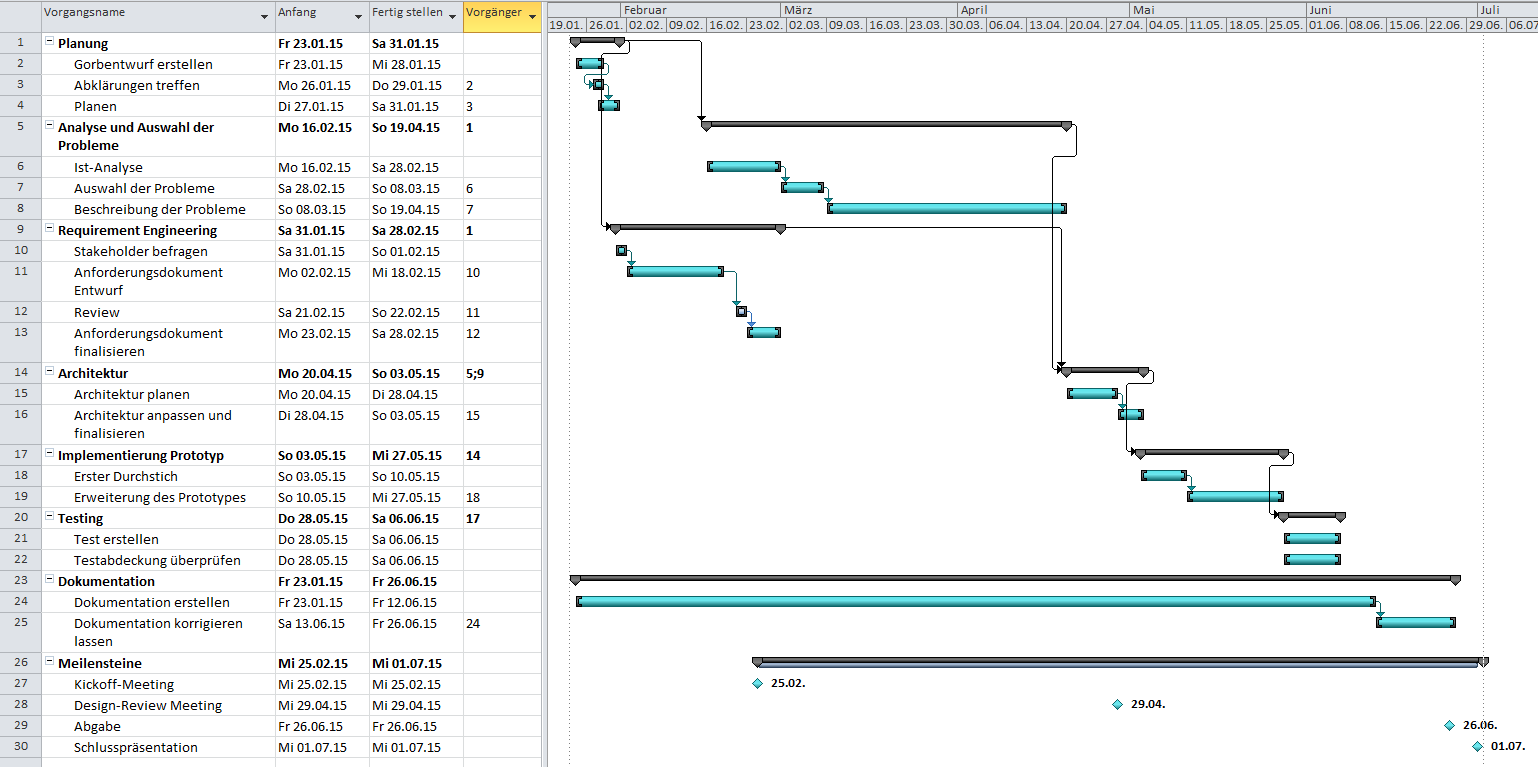
\includegraphics[scale=0.5]{images/project/projectplan.png}
\caption{Projektplan}
\label{fig:psp}
\end{figure}

\end{landscape}

\subsection{Zeitschätzung auf Arbeitspaketebene}
\begin{table}[ht]
\centering
  \begin{tabular}{ l | c | c }
	\hline
	\rowcolor{gray}
	\textbf{Arbeitspaket}					&	\textbf{Schätzung (h)}	& \textbf{Tatsächlich (h)}	\\ \hline
	Requirement Engineering					&	20			& 30	\\ \hline
	Reale Optimierungsprobleme suchen			&	50			& 70	\\ \hline
	Wissensaufbau Algorithmen				&	70			& 70	\\ \hline
	Architektur Planung						&	60			& 60	\\ \hline
	Prototyp Entwicklung					&	50			& 50	\\ \hline
	Tests								&	10			& 10	\\ \hline
	Dokumentation						&	120			& 120	\\ \hline \hline
	Total								&	380			& 410	\\ \hline
  \end{tabular}
   \caption{Zeitschätzung auf Arbeitspaketebene}\label{table:time_estimation}
\end{table}

\section{Risikoanalyse}\label{risikoanalyse}
Jedes Projekt birgt Risiken. Werden diese nicht am Anfang analysiert und über die gesamte Projektlaufzeit überwacht, kann es zu grossen Schwierigkeiten kommen. Die angewandten Methoden sind aus \cite{proj_mgmt_book} und aus dem dem Management Fach Projekt und Prozessmanagement bekannt.

\subsection{Risikoermittlung}\label{risikoermittlung}
Die Risikoermittlung wird zur Bestimmung und Folgenabschätzung möglicher Risiken angewendet.

\begin{table}[ht]
\centering
  \begin{tabular}{  p{5cm} | p{9cm} }
	\hline
	\rowcolor{gray}
	\textbf{Risiko}					&	\textbf{Mögliche Folgen}	\\ \hline
	Implementationsschwierigkeiten (fast keine Erfahrung in der Theoretischen Informatik)
								&	\begin{itemize}
										\item Zeitplan nicht einhaltbar
										\item Einige Anforderungen müssen zurückgestellt werden
										\item Projektarbeit kann nicht durchgeführt werden
									\end{itemize}	\\ \hline
	Zeitengpässe
								&	\begin{itemize}
										\item Zeitplan nicht einhaltbar
										\item Einige Anforderungen müssen zurückgestellt werden
										\item Projektarbeit kann nicht durchgeführt werden
									\end{itemize}	\\ \hline
	Mangelhaftes Endprodukt		
								&	\begin{itemize}
										\item Produkt muss überarbeitet werden, da keine Abnahme durch den Stakeholder erfolgt
									\end{itemize}	\\ \hline	
	Anforderungen nicht vollständig	
								&	\begin{itemize}
										\item Wichtige Funktionen stehen den Benutzern nicht zur Verfügung
									\end{itemize}	\\ \hline			
  \end{tabular}
   \caption{Risikoermittlung}
\end{table}

\subsection{Risikobewertung}
Das Schadensausmass und die Eintrittswahrscheinlichkeit der Risiken sind nach folgendem Schema bewertet worden:

\begin{table}[ht]
\centering
  \begin{tabular}{ l | p{5cm} | p{5cm} }
	\hline
	\rowcolor{gray}
	\textbf{Wert}					&	\textbf{Eintrittswahrscheindlichkeit} &	\textbf{Schadensausmass}	\\ \hline			
	1							&	sehr unwahrscheinlich		&	vernachlässigbar	\\ \hline
	2							&	unwahrscheinlich			&	spürbar		\\ \hline
	3							&	wenig wahrscheinlich		&	verkraftbar		\\ \hline
	4							&	ziemlich wahrscheinlich		&	gefährlich		\\ \hline
	5							&	sehr wahrscheinlich			&	katastrophal		\\ \hline
  \end{tabular}
   \caption{Risikobewertungsschema}
\end{table}

\FloatBarrier
Die Risiken aus der Risikobewertung (siehe \ref{risikoermittlung}) wurden anhand dieses Schemas bewertet.

\begin{equation*}
Risikofaktor = Eintrittswahrscheindlichkeit * Schadensausmass
\end{equation*}

\begin{table}[ht]
\centering
  \begin{tabular}{ l | p{4cm} | p{3cm} | c }
	\hline
	\rowcolor{gray}
	\textbf{Risiko}					&	\textbf{Eintrittswahrscheindlichkeit} &	\textbf{Schadensausmass} 	&	\textbf{Risikofaktor}\\ \hline			
	Implementationsschwierigkeiten			&	3					&	4			&	\textbf{12}	\\ \hline
	Zeitengpässe					&	2					&	5			&	\textbf{10}	\\ \hline
	Mangelhaftes Endprodukt				&	2					&	4			&	\textbf{8}	\\ \hline
	Anforderungen nicht vollständig			&	2					&	2			&	4		\\ \hline
  \end{tabular}
   \caption{Risikobewertung}
\end{table}

\subsection{Risikomatrix}
Anhand der Risikobeurteilung konnten die Risiken in eine Risikomatrix eingesetzt werden. Diese Matrix bietet einen guten Überblick über die Risiken und zeigt schnell, welche Risiken beachtet werden müssen.
\begin{figure}[h]
\centering
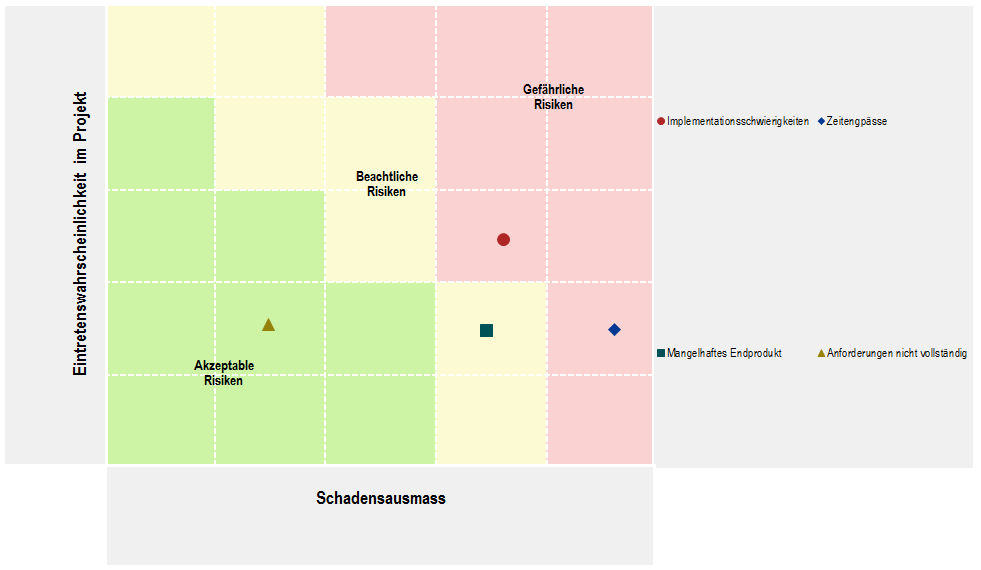
\includegraphics[scale=0.5]{images/excel/risikomatrix.png}
\caption{Risikomatrix}
\label{fig:risikomatrix}
\end{figure}

\subsection{Massnahmen}
Es wurden Massnahmen für die gefundenen Risiken gesucht und festgehalten. Die Massnahmen sind wiederum in vorbeugende Massnahmen und Eventualmassnahmen unterteilt.

\begin{table}[ht]
\centering
  \begin{tabular}{  l | p{4cm} | p{4cm} }
	\hline
	\rowcolor{darkgray}
	\textbf{Risiko}					&	\multicolumn{2}{|c|}{\textbf{Massnahmen}} \\ \hline
	\rowcolor{gray}
								&	Vorbeugende Massnahmen & Eventualmassnahmen	\\ \hline
	Implementationsschwierigkeiten
								&	\begin{itemize}
										\item Im Zeitplan genügen Reserver einrechnen
										\item Kontaktpersonen zum Thema suchen
										\item Zeitplan einhalten, pünktlich mit den Arbeiten beginnen
									\end{itemize}
								&	\begin{itemize}
										\item Betreuer / Schulleitung informieren
										\item Verschiebungsgesuch stellen
									\end{itemize}						\\ \hline
	Zeitengpässe
								&	\begin{itemize}
										\item Fixe Zeiten einplanen
										\item Tätigkeiten priorisieren
									\end{itemize}
								&	\begin{itemize}
										\item Verschiebungsgesuch stellen
									\end{itemize}	\\ \hline
	Mangelhaftes Endprodukt		
								&	\begin{itemize}
										\item Anforderungskatalog sauber erstellen
										\item Kunden laufend über den Stand des Produktes informieren
									\end{itemize}
								&	\begin{itemize}
										\item Lösung mit dem Kunden suchen
										\item Projekt verlängern
									\end{itemize}	\\ \hline	
	Anforderungen nicht vollständig	
								&	\begin{itemize}
										\item Review des Anforderungskataloges
										\item Kunden laufend über den Stand des Produktes informieren
									\end{itemize}
								&	\begin{itemize}
										\item Anforderungen werden aufgenommen und in einen nächsten Release geplant							
									\end{itemize}	\\ \hline			
  \end{tabular}
   \caption{Risikoanalyse - Massnahmen}
\end{table}


